\documentclass{article}
\usepackage{template/iclr2027_conference,times}
\usepackage{amsmath,amssymb,amsthm,booktabs,graphicx,longtable,hyperref,url}
\newcommand{\OptSyn}{6.51}
\newcommand{\OptSynSE}{0.09}
\newcommand{\OptReal}{2.32}
\newcommand{\OptRealSE}{0.09}
\newcommand{\SynNaiveCov}{83.95}
\newcommand{\SynAuditCov}{96.60}
\newcommand{\RealNaiveCov}{95.90}
\newcommand{\RealAuditCov}{96.35}
\newcommand{\SynFalseNaive}{10.85}
\newcommand{\SynFalseAudit}{0.10}
\newcommand{\RealFalseNaive}{0.00}
\newcommand{\RealFalseAudit}{0.00}
\newcommand{\MeanCorr}{0.783}
\newcommand{\RawMinAcc}{82.17}
\newcommand{\RawMaxAcc}{85.17}
\newcommand{\FormatFailures}{40}
\newcommand{\PromptTokens}{1,168,858}
\newcommand{\CompletionTokens}{1,282,295}
\newcommand{\InferenceMinutes}{40.6}
\newcommand{\Winner}{5}
\newcommand{\CardSelection}{87.50}
\newcommand{\CardAudit}{83.59}
\newcommand{\CardTruth}{84.50}
\newcommand{\CardLower}{77.33}
\newcommand{\CardUpper}{89.17}
\newcommand{\CardDeltaLower}{-3.67}
\newcommand{\CardDeltaUpper}{9.50}
\newcommand{\CardDelta}{2.33}
\newcommand{\CardPlus}{6}
\newcommand{\CardMinus}{2}

\newtheorem{proposition}{Proposition}
\newcommand{\E}{\mathbb E}
\newcommand{\Prob}{\mathbb P}
\newcommand{\ind}{\mathbf 1}
\title{Reporting a Selected Prompt:\\Winner Optimism, Finite-Pool Targets, and Conditional Audits}
\author{Anonymous authors}
\begin{document}
\maketitle
\begin{abstract}
A benchmark score used to choose a prompt is a selection statistic, not automatically an honest estimate of the chosen system. We study the discrepancy with known-truth experiments and a newly collected response cache: eight frozen prompts, 600 MMLU-Pro questions, and one supplied LLM endpoint. The central distinction is between a selected configuration's population accuracy, its accuracy on a fixed cohort, and its accuracy on the unselected remainder. These targets require different reference quantities. In the primary equal-quality simulation, winner optimism is \OptSyn{} percentage points and a nominal 95\% Wilson interval covers only \SynNaiveCov\%; a fresh exact audit covers \SynAuditCov\%. In the real fixed-cohort replay, optimism is \OptReal{} points and the corresponding coverages are \RealNaiveCov\% and \RealAuditCov\%: optimism does not force undercoverage in every setting. A finite-population audit can be mapped exactly back to cohort accuracy and paired baseline improvement. We give its conditional guarantee, including joint confidence allocation, and document a boundary setting in which a correlation-aware multiplier approximation fails. The empirical evidence is a fixed-family case study, not a population guarantee for this endpoint or a validation of arbitrary adaptive optimizers. All responses, seeds, and analyses are released.
\end{abstract}

\section{Introduction}
Automatic prompt selection creates a statistical dependency that ordinary benchmark reporting often hides. A researcher evaluates several configurations, chooses the highest-scoring one, and reports its score on the same questions. Even if every candidate has exactly the same true accuracy, selection can turn sampling noise into an apparent gain. The chosen system may genuinely improve, but a reused score alone cannot establish the size or even the sign of that improvement on new questions.

There are two distinct problems: estimating accuracy and deciding whether the selected system improves over a baseline. A confidence interval for one fixed prompt need not cover a prompt chosen using those same answers. Conversely, replacing a reused score with an independent-looking holdout score is insufficient unless the holdout's target and access history are specified. In a finite benchmark, an audit drawn without replacement from the unselected questions estimates the \emph{remainder}, not the original cohort. The distinction matters most when selection consumes a substantial fraction of the available questions.

This paper is an estimand-explicit statistical case study rather than a new general theory of post-selection inference. Its contributions are: (i) a controlled measurement of optimism, interval coverage, and false promotion under prompt dependence, candidate count, sample size, and true-quality gaps; (ii) a finite-pool reporting recipe that combines exact conditional auditing, a known-contribution transformation, and paired baseline comparisons; and (iii) an independently collected real-LLM cache exposing both the practical scale and limitations of these procedures. The underlying statistical ingredients are standard. The useful contribution is their explicit sampling contract, executable comparison, and stress testing rather than a claim to have invented sample splitting or the winner's curse.

A key scope limitation is stated upfront: the real experiment uses eight \emph{prespecified} prompts and one endpoint whose model alias cannot be independently authenticated. Its complete cache supports exact finite-cohort reference quantities, not an oracle for fresh-question population performance. Population coverage is evaluated only where population truth is known, in simulations. A restricted, direct-source literature protocol also prevents an exhaustive novelty assessment.

\section{Related work}
\paragraph{Prompt optimization and evaluation.}
\citet{shi2024} connect fixed-budget prompt selection to best-arm identification, emphasizing selection quality under a budget. That optimization objective differs from inference about the accuracy of the configuration ultimately selected. \citet{polo2024} estimate the distribution of performance across prompt variants, whereas the target here is the particular data-selected configuration. \citet{sclar2024} document sensitivity to meaning-preserving prompt-format changes and motivate reporting performance over plausible formats. Sensitivity and selection bias are different: true prompt-quality variation can exist without reused-score optimism, and optimism can exist with identical true qualities. MMLU-Pro expands answer choices and emphasizes more challenging reasoning questions \citep{wang2024}; it provides the real item frame for this case study.

\paragraph{Adaptive reuse and simultaneous inference.}
\citet{dwork2015} study validity under adaptively chosen analyses, and \citet{blum2015} address adaptive leaderboard reporting. Our fixed-family selection-only bound is much narrower than those general adaptive settings. A family-size bound cannot be applied merely by counting candidates generated after seeing the selection data. In contrast, a properly isolated fresh audit can condition on an arbitrarily complicated pre-audit search history. We do not implement or claim a replacement for privacy-based reusable holdouts or the Ladder.

\paragraph{Correlation-aware approximation.}
Gaussian multiplier methods approximate maxima of vector sums under conditions studied by \citet{cck2013}. This motivates sharing a resampling weight across the full vector of prompt outcomes for one item. It does not establish finite-sample validity for small, nearly degenerate correctness tables. We therefore compare the approximation to conservative simultaneous concentration and exact audit inversion, and explicitly retain its failures. Related-work statements here are grounded in the directly consulted abstracts of the permitted sources, not a comprehensive literature survey.

\section{What score is being estimated?}
\subsection{Population, cohort, remainder, and algorithm targets}
For a family of $K$ configurations fixed independently of the selection items, let $Y_i=(Y_{i1},\ldots,Y_{iK})$ be iid bounded item-outcome vectors, $p_j=\E Y_{ij}$, and $\widehat p_j=n^{-1}\sum_iY_{ij}$. The selector chooses $J=\arg\max_j\widehat p_j$ with a frozen tie rule. The selected-configuration population target is $p_J$. Dependence \emph{between prompts on the same item} is allowed; independence of item vectors is the population sampling assumption.

For a fixed binary response table with $N$ rows, write $\mu_j=N^{-1}\sum_{i=1}^N Y_{ij}$. A uniformly sampled selection set $S$, $|S|=n$, has score $s_j$. The unselected remainder $R=S^c$ has size $M=N-n$ and mean $\mu_{R,j}$. Pointwise, including after selection,
\begin{align}
 \mu_J&=\frac nN s_J+\frac MN\mu_{R,J},\label{eq:mapping}\\
 s_J-\mu_{R,J}&=\frac NM(s_J-\mu_J).\label{eq:gap}
\end{align}
Thus the often-reported selection-minus-heldout gap is scaled relative to selection-minus-cohort optimism. The remainder target itself changes with $S$. Neither quantity automatically equals population accuracy. Finally, $\E_S[p_{J(S)}]$ is the \emph{search algorithm's} expected performance at a specified search-sample size, not the accuracy of its particular final winner. Outer resampling or nested cross-validation must not silently substitute this different estimand.

\subsection{Fixed-family optimism and its boundary}
\begin{proposition}[Fixed-family expected optimism]\label{prop:optimism}
For iid item vectors in $[0,1]^K$ and an empirical maximizer from an independently fixed family,
\[
0\leq\E[\widehat p_J-p_J]\leq\sqrt{\frac{\log K}{2n}}.
\]
For $K=1$ the expectation is zero. The same statement holds for $s_J-\mu_J$ under uniform sampling without replacement from a fixed cohort.
\end{proposition}
For the lower bound, $\E\max_j\widehat p_j\geq\max_jp_j\geq\E p_J$. For the upper bound, each centered column mean has moment-generating function at most $\exp(\lambda^2/(8n))$. A log-sum-exp bound followed by optimization over $\lambda$ proves the result; no column independence is used. Appendix~\ref{app:proofs} supplies details. The bound concerns an expectation, not every observed score, and is not a correction to subtract from each winner.

A selection-only interval valid for an arbitrary choice \emph{within this fixed family} uses radius
\begin{equation}
 r_H=\sqrt{\frac{\log(2K/\alpha)}{2n}}.\label{eq:hoeffding}
\end{equation}
A two-sided union bound gives simultaneous coverage at least $1-\alpha$, for iid items or uniform sampling without replacement. This can be imprecise, but it makes the family assumption visible.

The assumption cannot be replaced with ``$K$ configurations were generated.'' For continuous iid inputs with label always one, a data-dependent classifier that predicts one only on the observed inputs has selection accuracy one and population accuracy zero. Counting just that single generated configuration would give $K=1$, contradicting an unrestricted extension. This is an expressivity counterexample, not a demonstration that the particular LLM prompts in this study memorize data. It explains why unrestricted adaptive generation requires fresh auditing or a separately justified complexity argument.

\section{Conditional audit reporting}
\subsection{Freeze the winner, then sample the audit}
Let $H$ be the complete pre-audit history. Freeze the chosen configuration, baseline, scoring rule, audit size, targets, and confidence allocation before exposing audit answers. For a finite cohort, $S$ must include \emph{every} item whose information influenced search. Conditional on $H$, assume fixed potential binary outcomes for the frozen configurations on the genuinely unaccessed remainder, and sample $m$ audit items uniformly without replacement. The chosen prompt's audit successes then obey
\[
 X\mid H\sim\operatorname{Hypergeom}(M,T,m),\qquad T=M\mu_{R,J}.
\]
Accept an integer candidate $t\in\{0,\ldots,M\}$ if
\begin{equation}
 \Prob_t(X\geq x)\geq\alpha/2,\qquad
 \Prob_t(X\leq x)\geq\alpha/2.\label{eq:inversion}
\end{equation}
The hull of the accepted $t/M$ values is an exact, possibly conservative, $1-\alpha$ remainder interval $[L_R,U_R]$. Each inclusive tail is a valid discrete $p$-value; a union bound proves conditional coverage. Applying equation~\eqref{eq:mapping} to its endpoints gives
\begin{equation}
 I_{\rm cohort}=\frac nN s_J+\frac MN[L_R,U_R],\label{eq:poolci}
\end{equation}
with exactly the same coverage event for $\mu_J$. If final-configuration scores on previously accessed items are unknown, that offset must first be evaluated; a nominal ``training subset'' cannot replace the complete access set.

For genuinely fresh iid audit items independent of $H$, the corresponding count is binomial and the same tail inversion gives a Clopper--Pearson interval for $p_J$. This guarantee permits arbitrary pre-audit adaptive search. It does not permit audit-feedback reranking, adaptive stopping, or repeated reporting with the same unadjusted audit. It also does not turn a finite-cohort sample into a population sample. Conditional uniformity, not mere item disjointness, is the essential finite-pool requirement.

\subsection{Paired improvements and two headline claims}
On the same audit items, count $D^+=\ind\{Y_J=1,Y_0=0\}$ and $D^-=\ind\{Y_J=0,Y_0=1\}$ against the immutable baseline. Their marginal proportions $q^+,q^-$ satisfy $\Delta=q^+-q^-$. Given two exact marginal intervals each with failure budget $\beta/2$, an interval for improvement is
\begin{equation}
 I_\Delta=[L_+-U_-,\ U_+-L_-].\label{eq:pair}
\end{equation}
The discordance counts need not be independent: Bonferroni suffices. In the finite cohort, apply the analogue of equation~\eqref{eq:poolci} using the observed selection difference. For a self-comparison the difference and its interval are exactly zero. Promote only if the lower endpoint for the \emph{named target} exceeds zero. False promotion when the true selected-minus-baseline effect is nonpositive implies noncoverage, and is therefore controlled by $\beta$ under the audit contract.

Two separately valid 95\% intervals do not constitute a joint 95\% report. Our final replay report card assigns $\alpha_a=0.025$ to accuracy and $\alpha_\Delta=0.025$ to improvement. Each discordance marginal consequently uses failure budget $0.0125$. The two headline claims have joint coverage at least 95\%. Method-comparison experiments instead assess separate marginal 95\% accuracy and improvement claims; they do not assert a joint 95\% guarantee for every entry or grid cell.

\subsection{Approximate and no-audit alternatives}
We compare six accuracy procedures: naive winner Wilson; simultaneous Hoeffding; a Gaussian row-multiplier maximum; a guarded multiplier; audit Wilson; and exact audit inversion. The multiplier centers each selection column, shares Gaussian weights across items' prompt vectors, and takes the 95th percentile of the maximum absolute mean deviation. It uses sample-variance scaling and, for a fixed cohort, finite-population factor $\sqrt{1-n/N}$. A covariance eigendecomposition generates the identical conditional Gaussian distribution efficiently. Its radius is \emph{approximate}, including with the finite-population factor. The guard uses Hoeffding if $n<64$ or any column has fewer than five successes or failures; otherwise it uses the multiplier. This is a heuristic, not a new coverage theorem. Both audit intervals are mapped to cohort accuracy in real-cache comparisons, ensuring like-target comparisons.

\section{Experimental design}
\paragraph{Frozen contract and metrics.}
Before acquiring scored responses, we froze the cohort, prompt family, parser, sample-size grids, seeds, primary metrics, and token/call ceilings. The primary setting is $K=8,n=64,m=128$, with 2,000 repeated item selections. Its iid population cell has $p_j=0.7$ for all prompts and latent $\rho=0.5$. Metrics are mean optimism, accuracy coverage and width, and false promotion against prompt P0. We report Monte Carlo standard errors (MCSE), not only aggregate means. For the real cache these errors are conditional on that fixed table, \emph{not} uncertainty over new benchmarks or model generations. Confidence coverage in simulations is checked against known $p_J$; real-cache coverage is checked against the exact cached $\mu_J$.

\paragraph{Known-truth experiments.}
For each iid item, generate $Z_j=\sqrt{\rho}Z_0+\sqrt{1-\rho}\epsilon_j$ and $Y_j=\ind\{Z_j\leq\Phi^{-1}(p_j)\}$. The core grid crosses $n\in\{16,32,64,128\}$, latent $\rho\in\{0,0.5,0.9\}$, and last-prompt quality gap $\delta\in\{0,0.01,0.05\}$, with other prompts at $p_0=0.7$. This gives 36 core cells. Fourteen further cells stress candidate counts 1--16, boundary accuracies, and exact duplicates. Seven sensitivity cells vary audit size, multiplier dependence, and resampling budget; one fixed synthetic finite pool completes 58 settings. Except four multiplier-budget checks using the first 200 replicates, each uses 2,000 repetitions. The latent correlation parameter is not the observed binary correlation. True gaps and dependence are controlled separately; no empirical ``effective number of prompts'' is inferred from correlation alone.

\paragraph{Real LLM acquisition.}
The pinned MMLU-Pro revision is \texttt{b189ec765aa7ed75c8acfea42df31fdae71f97be}. An outcome-blind, approximately proportionally stratified sample provides 600 test questions across 14 subjects. Replay sampling within this cohort is uniform, not stratified. All available choices are retained: the original test frame has 3--10 choices rather than universally ten. No gold answers or solution explanations enter requests. Eight zero-shot prompts form a $2\times2\times2$ family: neutral versus subject-expert framing, direct versus option-elimination instruction, and answer-only versus a brief explanation. Every prompt ends with the same final-answer marker requirement. The full family and item IDs are supplied.

The supplied compatible API serves alias \texttt{gpt-5.6-luna}; we verified actual text completions but cannot independently verify model weights, release, training data, or provider routing. We request temperature zero and \texttt{max\_tokens=192}, issue the 4,800 item--prompt requests in shuffled order at concurrency eight, and cache raw requests, responses, hashes, usage, and timestamps. The requested maximum was not an enforceable cap on provider-reported completion usage; its semantics are discussed below. Strict parsing requires exactly one valid final \texttt{ANSWER: <letter>} marker. Content failures count as incorrect and are never regenerated for correctness. The frozen baseline is P0; ties choose the smallest ID. This is exhaustive score-based selection from a small fixed family, not a reproduction of DSPy, MIPRO, or adaptive prompt generation.

\paragraph{Diagnostics and uncertainty.}
Small-pool enumeration checks hypergeometric coverage and the entire selection--audit mapping; parser fixtures, duplicate-prompt limits, and self-comparison checks precede analysis. The implementation passes these checks. Guaranteed-method undercoverage is screened with one-sided binomial checks and Holm adjustment across the synthetic cells; no rejection occurs. All cells, including null and failed approximations, remain in the supplied tables. Confirmatory grids are descriptive comparisons, not a search for statistically significant settings. Additional sensitivity outputs do not license a post-hoc best reporting rule.

\section{Results}
\subsection{Optimism depends on sample size, dependence, and the target}
Figure~\ref{fig:optimism} shows that in the equal-quality synthetic setting, mean optimism decreases as selection size increases and as prompts become more correlated. Perfectly duplicate prompts select the baseline under our tie rule and do not create additional search gain. In the primary simulation, optimism is \OptSyn{} pp (MCSE \OptSynSE{} pp). Increasing candidate count provides additional opportunities to select noise; true-quality gaps affect both selection regret and optimism, but the small tested gaps do not produce a uniformly monotonic change. The independent equal-quality limit also admits a binomial maximum calculation, supplied alongside simulations as an analytic check.

\begin{figure}[t]
\centering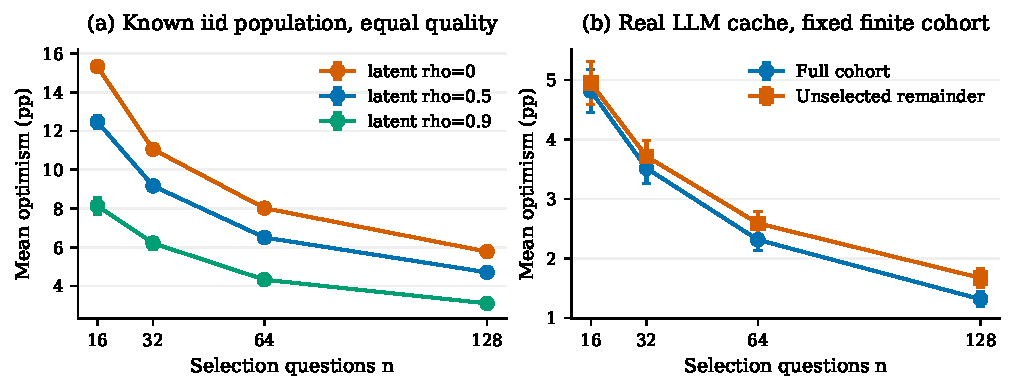
\includegraphics[width=\linewidth]{artifacts/figures/optimism.pdf}
\caption{Winner optimism relative to known iid population accuracy (left) and exact real-cache targets (right). Error bars are $1.96\times$ conditional MCSE, not population uncertainty for the real endpoint. The remainder curve is larger by the exact $N/(N-n)$ factor; it is not a competing estimate of the same parameter.}\label{fig:optimism}
\end{figure}

For the real response table, prompt accuracies range from \RawMinAcc\% to \RawMaxAcc\%, with mean off-diagonal binary correctness correlation \MeanCorr{}. At $n=64$, mean cohort optimism is \OptReal{} pp (MCSE \OptRealSE{} pp). Each replay's remainder is unseen by its selector, so this also measures transfer to questions not used by that selection process through equation~\eqref{eq:gap}. It does not quantify performance on an externally sampled, contamination-free population. The smaller real family, its unequal accuracies, and its shared item errors prohibit attributing its optimism to candidate count alone. Nested candidate-count ablations also change family composition and are labeled accordingly.

\subsection{Coverage, precision, and an approximate-method failure}
\begin{table}[t]
\caption{Primary setting $K=8,n=64,m=128$, 2,000 repetitions. Coverage is percent $\pm$ one plug-in MCSE (percentage points); width is in percentage points. Zero MCSE at observed 100\% coverage is not certainty: exact binomial Monte Carlo intervals are also supplied in the CSV. Targets: known $p_J$ for iid simulation and exact $\mu_J$ for the real cache. Methods use different additional-data budgets: audit methods consume $m$ fresh audit responses for accuracy. Guarded and raw multiplier agree when the guard never fires.}\label{tab:primary}
\centering\small\begin{tabular}{lrrrr}
\toprule
& \multicolumn{2}{c}{Iid population} & \multicolumn{2}{c}{Real finite cohort} \\
Method & Coverage & Width & Coverage & Width \\
\midrule
Naive & 83.95 $\pm$ 0.82 & 20.28 & 95.90 $\pm$ 0.44 & 16.67 \\
Hoeffding & 99.95 $\pm$ 0.05 & 41.71 & 100.00 $\pm$ 0.00 & 34.87 \\
Multiplier & 97.30 $\pm$ 0.36 & 30.88 & 96.50 $\pm$ 0.41 & 21.63 \\
Guarded & 97.30 $\pm$ 0.36 & 30.88 & 99.20 $\pm$ 0.20 & 22.12 \\
Audit Wilson & 94.60 $\pm$ 0.51 & 15.58 & 97.55 $\pm$ 0.35 & 11.33 \\
Audit exact & 96.60 $\pm$ 0.41 & 16.40 & 96.35 $\pm$ 0.42 & 10.38 \\
\bottomrule
\end{tabular}
\end{table}
The naive interval has primary coverage \SynNaiveCov\% in simulation and \RealNaiveCov\% in the real finite-cohort replay (Table~\ref{tab:primary}). The latter is not evidence of undercoverage: this real setting retains nominal marginal coverage despite positive score optimism. Conservative binomial approximation for without-replacement sampling, strong shared errors, and family-quality differences can offset selection effects; this study does not causally separate their contributions. Larger $n$ reduces absolute optimism but does not automatically restore nominal coverage: standard errors also shrink, and discrete Wilson coverage need not vary monotonically with $n$. Exact audits achieve \SynAuditCov\% and \RealAuditCov\% for the corresponding targets. Their conservative validity is a property of the sampling design and inversion, not a conclusion drawn from agreement with a noisy heldout score. Hoeffding is wider but does not require post-selection approximation.

\begin{figure}[t]
\centering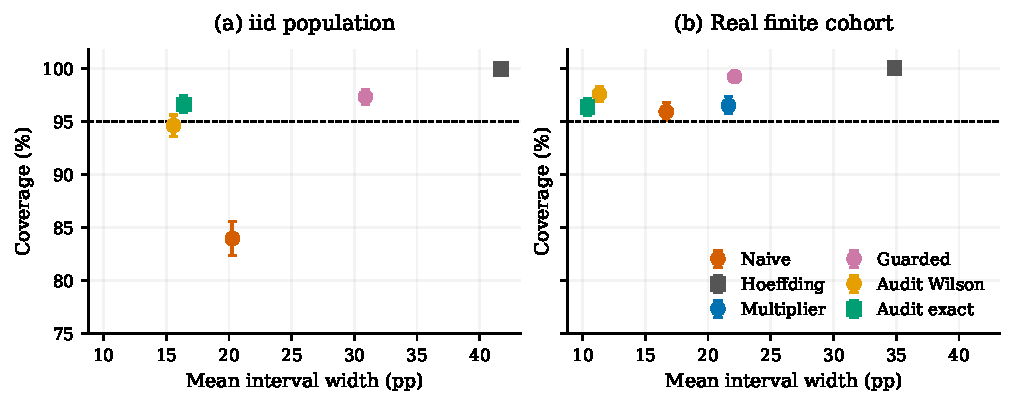
\includegraphics[width=\linewidth]{artifacts/figures/coverage_width.pdf}
\caption{Coverage--precision trade-off for the two primary targets. Square markers denote the finite-sample-guaranteed procedures under their stated designs; circles denote approximate procedures. The horizontal line is 95\%. Narrowness without coverage is not improved reporting. Primary guarded/raw multiplier points can overlap.}\label{fig:coverage}
\end{figure}

The multiplier can be more informative than a worst-case union bound, but this benefit is conditional. In the predeclared boundary stress $p_0=0.95,n=16,\rho=0.9$, its measured coverage is 82.50\% over 2,000 repetitions. Nearly constant columns can yield an estimated radius of zero even when true accuracy is below one. This is a statistical degeneration, not merely too few Gaussian draws. The guard reverts to Hoeffding throughout this stress, recovering conservativeness at a substantial width cost. The supplied $B=999$ versus $3,999$ checks on paired subsets characterize numerical quantile noise but do not turn an approximate method into an exact one.

\begin{figure}[t]
\centering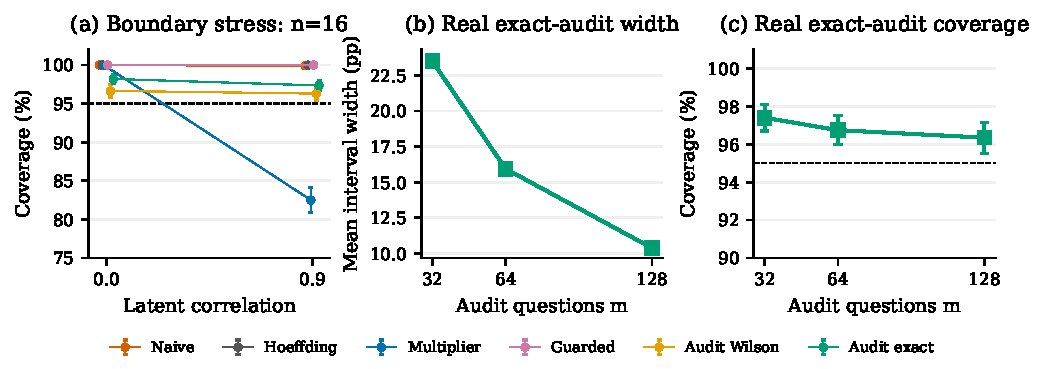
\includegraphics[width=\linewidth]{artifacts/figures/failure_precision.pdf}
\caption{A predeclared near-boundary failure of multiplier approximation (left) and the cost of exact real-cache auditing as $m$ increases (middle/right). The guard uses the conservative fallback at $n=16$. Full parameter grids and no-FPC/independent-multiplier sensitivities are released, not selected for favorable coverage.}\label{fig:failure}
\end{figure}

\subsection{Decisions and the reporting contract}
Under the all-equal primary simulation, a naive paired normal interval computed on selection answers falsely promotes a winner in \SynFalseNaive\% of repetitions; the exact paired audit rule falsely promotes in \SynFalseAudit\%. This is an unconditional false-promotion probability against the predeclared baseline, not false discovery rate. The exact paired construction is intentionally conservative: low false promotion can coexist with low power. In the real-cache primary setting, the analogous false-promotion frequencies relative to exact finite-cohort effects are \RealFalseNaive\% and \RealFalseAudit\%; these are conditional replay quantities and depend on which winners have nonpositive true effects. In fact P0 is the lowest-accuracy prompt on this cache: the nonpositive-effect cases are self-comparisons. The zero real false-promotion frequency is therefore not a real-data type-I stress test; the equal-quality simulations supply that evidence.

A single precommitted replay illustrates the report format. Its winner is P\Winner{}, selection score \CardSelection\%, audit score \CardAudit\%, and exact cohort reference \CardTruth\%. The joint-95\% report-card accuracy interval is [\CardLower,\CardUpper]\%, and its paired cohort-improvement interval is [\CardDeltaLower,\CardDeltaUpper] pp (true cached difference \CardDelta{} pp). Audit discordances are \CardPlus{} positive and \CardMinus{} negative. This is explicitly a \emph{replay illustration}: the investigator could access the complete cache. It is not evidence that a prospectively blinded audit was operationally enforced. A guarantee for future deployment requires that enforcement, not just reuse of this report format.

\section{Discussion and limitations}
\paragraph{What can be concluded.}
A selected score and an honest performance report answer different questions. The studied gap can change decisions even when there is no true improvement. Its size depends jointly on search breadth, prompt-error dependence, item count, true-quality gaps, tie handling, and the target. Our reporting recommendation is to disclose the reused score as a selection statistic, identify the frozen winner and complete search history, publish a fresh audit with a named sampling target, and use a paired comparison if claiming improvement. If no new items are available, a conservative simultaneous interval is defensible only for an independently fixed encompassing family; a narrow approximate interval should not be substituted without qualifications.

\paragraph{Limits of the evidence.}
The real setting contains one API alias, one benchmark cohort, one output per item--prompt pair, and only eight zero-shot templates. It does not measure prompt-generation adaptivity, multistage pipelines, model-family variation, or long-chain-of-thought optimization. Temperature zero does not prove deterministic generation. Cache replay conditions on generation noise and cannot certify fresh-response accuracy. Benchmark pretraining contamination, label errors, and distribution shift remain unresolved. Uniform inference within the selected stratified cohort does not establish population or full-MMLU-Pro coverage. A larger independent sample and a prospectively sealed audit are the smallest useful next validation, not an implication of the present result.

\paragraph{Cost and incompleteness.}
Acquisition used no GPU and completed in \InferenceMinutes{} minutes, reporting \PromptTokens{} prompt tokens and \CompletionTokens{} completion tokens. There were \FormatFailures{} parsing failures, all retained in scoring. These are endpoint-reported usage counts, not independently tokenized or billed quantities. In 1,292 calls the reported completion usage exceeded the requested 192-token maximum (largest 5,521), so the nominal product of calls and requested limit was not a hard usage cap. Unexposed reasoning or unsupported parameter semantics could explain this; the endpoint does not permit verification. No tariff or balance was exposed, so currency expenditure is unknown; bounded calls and observed usage replace an unverifiable dollar-budget claim. We report measured CPU runtimes and all reruns in the reproducibility log. One measured complete offline reproduction pass (tests, all simulations, real-cache replay, figures, budget sensitivity, report, compilation, and verification) took 127.6 seconds wall time and 127.4 CPU seconds, with peak child RSS 433.4 MiB. This excludes original inference, prior development/reruns, source retrieval, and agent compute; it is not a fabricated total-project compute estimate. All measured commands are recorded in \texttt{artifacts/reproduction\_resources.json}. The final demonstration lacks investigator blinding, and adaptive optimizers and external-population replication were not run. These limits prevent broad claims about the severity of contemporary benchmark overfitting or superiority over adaptive-data-analysis mechanisms.

\section{Conclusion}
Reusing the data that selected a configuration changes the interpretation of its score. Known-truth simulations demonstrate optimism, undercoverage, and false promotion; one real LLM response cache confirms a finite-cohort discrepancy under a modest fixed-family search. Conditional exact auditing offers a transparent alternative, provided the access contract, finite-versus-population target, and joint confidence budget are respected. It trades additional evaluation and potentially conservative intervals for interpretable evidence, rather than promising a universal correction to an automatically optimized score.

\section*{AI use statement}
This research deliverable was produced unattended by an AI research assistant, including study planning, mathematical arguments, implementation, source consultation, analyses, figures, interpretation, and manuscript drafting; auxiliary AI agents provided planning, proof critique, and writing feedback. Synthetic outcomes were generated by the supplied numerical code, not invented by language-model narration. The real benchmark answers were generated by the separately queried endpoint described in Section~5. Programmatic tests and an AI-assisted adversarial audit were performed, but no human scientific verification occurred. This disclosure does not assert human authorship, acceptance, or actual conference submission. Human authors taking responsibility would be required before submission.

\section*{Ethics statement}
The study uses public multiple-choice questions and no recruited human subjects. Dataset licensing, benchmark contamination, unsupported provider identity claims, and misleading statistical reporting are relevant concerns. No private credentials are released. The restricted-source protocol intentionally avoids a prohibited prior paper and its discussion; consequently novelty cannot be certified. No topical discovery searches were performed. No prohibited-content encounter was recognized.

\section*{Reproducibility statement}
All raw completions, item IDs, frozen prompts, deterministic scoring, seed namespaces, dataset revision, analysis scripts, measured usage, failed-run notes, and plotting/table-generation commands accompany the paper. Appendix~\ref{app:repro} and \texttt{README.md} map every result to its generating script. Fresh inference depends on endpoint availability; the released cache reproduces statistical results without network access.

\bibliography{references}
\bibliographystyle{template/iclr2027_conference}
\clearpage
\appendix
\section{Proof details and target checks}\label{app:proofs}
\subsection{Expected optimism and concentration}
Let $Z_j=\widehat p_j-p_j$. For a centered variable with support length one, the logarithm of its moment-generating function is zero with zero derivative at the origin; its second derivative is the variance under exponential tilting and is bounded by $1/4$. Integrating twice gives $\log\E e^{t(Y-\E Y)}\leq t^2/8$. Independence across items implies $\E e^{\lambda Z_j}\leq e^{\lambda^2/(8n)}$. Consequently,
\[
\E Z_J\leq\E\max_j Z_j\leq\frac1\lambda\log\sum_j\E e^{\lambda Z_j}
\leq\frac{\log K}{\lambda}+\frac{\lambda}{8n}.
\]
Choosing $\lambda=\sqrt{8n\log K}$ proves the upper bound for $K>1$. For $K=1$, unbiasedness gives zero directly. The lower bound follows because $\E\widehat p_J=\E\max_j\widehat p_j\geq\max_jp_j\geq\E p_J$. The lower bound requires empirical maximization; arbitrary choice within the family preserves only the upper bound. Neither part requires equal true accuracies or independent columns.

For without-replacement sampling from a fixed cohort, set $a_i=\exp\{\lambda(Y_{ij}-\mu_j)/n\}$. The sample-mean exponential moment is the normalized elementary symmetric mean of degree $n$ of these positive $a_i$. This is at most $(N^{-1}\sum_i a_i)^n$: pairwise averaging at fixed sum increases their product and does not decrease the elementary symmetric polynomial, whose maximum is attained at equal entries. Applying the preceding bounded-variable moment bound to one uniformly drawn cohort item gives the same $e^{\lambda^2/(8n)}$ bound. Unbiasedness and the maximum argument then apply to $s_J-\mu_J$. Chernoff's argument on both tails, followed by a union bound over the fixed family, gives equation~\eqref{eq:hoeffding}.

For independent equal-quality Bernoulli columns, the exact expectation used in the analytic diagnostic is
\[
\E\max_j\widehat p_j=\frac1n\sum_{x=0}^{n-1}\{1-F_{\operatorname{Binom}(n,p)}(x)^K\}.
\]
For dependent or unequal-quality columns this formula is not used.

The distinction between remainder and cohort is essential. A two-item fixed table with rows $(1,0)$ and $(0,1)$, selected on one item, always has winning score one, cohort mean one half, and remainder mean zero. Its remainder optimism is one, exceeding the unscaled bound $\sqrt{\log2/2}$. Equation~\eqref{eq:gap} explains the difference; it is not a failure of the fixed-cohort theorem.

\subsection{Conditional inversion and joint allocation}
For the true finite remainder count $T$, the inclusive upper-tail probability $\Prob_T(X\geq X_{\rm obs})$ is a valid discrete $p$-value: the event that it is below $u$ is an upper tail with probability at most $u$. The same holds for the lower tail. Thus the probability that either condition in equation~\eqref{eq:inversion} removes $T$ is at most $\alpha$. Taking the endpoint hull cannot decrease coverage. This includes boundary counts and a census $m=M$. A positive affine map preserves the coverage event, proving equation~\eqref{eq:poolci}. For iid fresh audit items, replace the hypergeometric law by the conditional binomial law; identical reasoning gives Clopper--Pearson.

For the paired effect, each discordance marginal has the appropriate hypergeometric or binomial sampling law. With probability at least $1-\beta$, both $q^+$ and $q^-$ lie in their intervals, regardless of their dependence. Subtraction then gives equation~\eqref{eq:pair}. The finite-cohort transformation is $\Delta_{\rm cohort}=(n/N)d_S+(M/N)\Delta_R$. For each history with $\Delta(H)\leq0$, positive lower bound implies noncoverage, so
\[
\Prob\{\mathrm{promote},\Delta(H)\leq0\}\leq\beta\Prob\{\Delta(H)\leq0\}\leq\beta.
\]
For the report card, failure of either headline interval is bounded by $0.025+0.025=0.05$; each paired marginal uses budget $0.025/2=0.0125$. In comparison plots the accuracy and improvement claims each receive $0.05$ separately, not jointly. The implementation's small floating-point relaxation of tail thresholds enlarges the accepted integer set; numerical tests are checks of code, not substitutes for these proofs.

Arbitrary pre-audit history is allowed only if conditional uniformity survives that history. Future audit membership cannot be exploited by search, and the audit cannot be used to choose baselines, rerank configurations, select the reporting rule, or decide when to stop. In a stochastic-generation setting, condition additionally on the full fixed response table if it was generated independently of audit sampling. Otherwise the finite-table proof does not automatically apply.

\section{Acquisition and reproducibility contract}\label{app:repro}
\paragraph{Data.}
The raw pinned test and validation parquet files and Hugging Face tree metadata are included. Only test questions enter the primary cohort. The preparation script outcome-blindly excludes conflicting duplicate question--option keys and retains the first consistent exact normalized duplicate; it records exclusions and category allocation. Labels are not relabeled using model answers. The validation split is downloaded for provenance but is not used as few-shot context or tuning data. Near-duplicate questions and pretraining contamination are not exhaustively resolved.

\paragraph{Prompts and parsing.}
IDs increase with expert framing fastest, then elimination, then explanation. The neutral prefix is ``Answer the following multiple-choice question.''; expert framing is ``You are a careful subject-matter expert in \{category\}.'' Direct instruction is ``Choose the single best answer.''; elimination is ``Compare the options and eliminate incorrect alternatives.'' Answer-only asks ``Return only your final answer.''; explanation asks for at most 50 words followed by the answer. All end with ``End with exactly one final line in this format: ANSWER: <letter>.'' The exact assembled strings are in \texttt{data/config.json}; question and all original options follow. A missing, conflicting, non-final, or out-of-range marker counts incorrect. Only transport failures can be retried; scoring failures cannot. All raw content remains available for alternative \emph{exploratory} scoring without overwriting the frozen analysis.

\begin{table}[h]
\caption{Complete real prompt cache; fixed scoring includes all parse failures.}\label{tab:prompts}
\centering\small\begin{tabular}{rrrrr}
\toprule
Prompt & Correct / 600 & Accuracy (\%) & Parse failures & Mean reported comp. tokens \\
\midrule
P0 & 493 & 82.17 & 4 & 225.5 \\
P1 & 502 & 83.67 & 3 & 252.1 \\
P2 & 494 & 82.33 & 8 & 256.4 \\
P3 & 498 & 83.00 & 8 & 294.4 \\
P4 & 511 & 85.17 & 2 & 263.4 \\
P5 & 507 & 84.50 & 4 & 273.0 \\
P6 & 502 & 83.67 & 5 & 277.8 \\
P7 & 495 & 82.50 & 6 & 294.6 \\
\bottomrule
\end{tabular}
\end{table}

\paragraph{Seeds and sampling.}
NumPy default generators use separate integer namespaces: cohort 2201, simulation 1101, replay 3301, report-card replay 4401, multiplier 5501, and request ordering 6601. Synthetic scenario keys receive stable SHA256-derived offsets, not Python's process-randomized hash. Core $n$ comparisons share prefixes of generated item vectors. Replays use independent uniform permutations from the same frozen cohort; $n,m$ comparisons share permutations. Candidate subsets are P0 for $K=1$, P0/P7 for $K=2$, P0/P3/P4/P7 for $K=4$, and all prompts for $K=8$. Their composition differs, so the real $K$ contrast is not a causal isolation of search breadth.

\paragraph{Artifacts and commands.}
\texttt{code/prepare.py} downloads no external answers and freezes metadata; \texttt{code/collect.py} makes actual endpoint calls and saves \texttt{data/responses.jsonl}. \texttt{tests/test\_statistics.py} validates interval primitives. \texttt{code/run\_experiments.py synthetic} generates all synthetic settings, analytic checks, and guarantee diagnostics; its \texttt{real} mode rebuilds and verifies all scores, replays finite-pool selection, and generates the report card. \texttt{code/plot\_results.py} alone generates every paper figure, all empirical LaTeX tables, and all empirical-number macros. The README gives exact invocation order and locked dependency versions. The released cache permits offline result reproduction, while a fresh endpoint run need not reproduce token-level outputs or identical accuracy.

\paragraph{Implementation and failed attempts.}
A first synthetic run exposed a Monte Carlo pairing bug in the reduced-repetition multiplier-budget sensitivity; its Gaussian arrays did not share the first 200 vectors of the main run. The generator was repaired to draw the full 2,000-vector set before taking a prefix, and all settings were rerun. This changed pairing, not the data-generating model or primary analysis. Two source-agent calls ended with provider overload after retrieving allowed files; these files were subsequently inspected directly. The final audit is not prospectively blinded. The complete deviation ledger and measured execution logs accompany the code. No adaptive optimizer, external population replication, or human review is represented as completed.

\section{Complete grids and ablations}
\begin{table}[h]
\caption{Predeclared real-cache ablations at $n=64$. Coverage is percent; width is pp. Exact audit targets the full cohort throughout. Changing the multiplier dependence/FPC leaves selection and audit data unchanged.}\label{tab:ablations}
\centering\small\begin{tabular}{lrrrr}
\toprule
Setting & Optimism (pp) & Naive cov. & Mult. cov. & Exact width \\
\midrule
K=1 & -0.15 & 96.50 & 95.30 & 10.73 \\
K=2 & 1.12 & 97.00 & 95.65 & 10.73 \\
K=4 & 1.49 & 96.85 & 95.80 & 10.33 \\
K=8 (primary) & 2.32 & 95.90 & 96.50 & 10.38 \\
m=32 & 2.32 & 95.90 & 96.50 & 23.50 \\
m=64 & 2.32 & 95.90 & 96.50 & 15.94 \\
Independent multipliers & 2.32 & 95.90 & 97.45 & 10.38 \\
Multiplier without FPC & 2.32 & 95.90 & 97.15 & 10.38 \\
\bottomrule
\end{tabular}
\end{table}
\begin{figure}[h]
\centering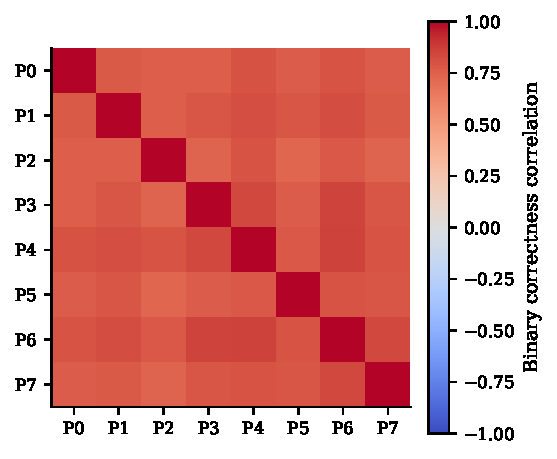
\includegraphics[width=.55\linewidth]{artifacts/figures/correlation.pdf}
\caption{Correctness correlations of all eight prompts on the fixed real cohort. These are descriptive cache quantities, not latent Gaussian parameters or evidence for an ``effective'' multiplicity correction.}\label{fig:corr}
\end{figure}
The following core-grid table is supplemented by \texttt{artifacts/synthetic\_summary.csv}, which includes all 58 settings, all six accuracy methods, MCSEs, widths, degeneracy/fallback frequencies, and paired-decision quantities. \texttt{artifacts/replications/} retains per-repetition arrays, allowing paired uncertainty calculations and independent metric checks. Coverage in the table is percent, optimism is pp, and false promotion refers to the naive paired selection-data rule. The exact-audit paired false-promotion results and the frequency of nonpositive effects appear separately in the CSV; they are not silently conditioned on selecting a harmful winner.
\begingroup\small\begin{longtable}{rrrrrrrr}
\caption{Complete core synthetic grid; optimism in pp, coverage and false promotion in percent.}\label{tab:core}\\
\toprule
$n$ & $\rho$ & $\delta$ & Optimism & Naive & Mult. & Exact & False prom. \\
\midrule\endhead
16 & 0 & 0 & 15.33 & 81.40 & 99.65 & 96.25 & 15.40 \\
16 & 0 & 0.01 & 15.38 & 81.00 & 99.65 & 96.30 & 14.10 \\
16 & 0 & 0.05 & 15.37 & 82.50 & 99.80 & 95.90 & 14.00 \\
16 & 0.5 & 0 & 12.47 & 86.90 & 98.25 & 96.70 & 11.50 \\
16 & 0.5 & 0.01 & 12.71 & 84.25 & 97.60 & 96.80 & 11.70 \\
16 & 0.5 & 0.05 & 12.92 & 83.65 & 97.75 & 97.10 & 10.95 \\
16 & 0.9 & 0 & 8.14 & 90.25 & 95.75 & 96.80 & 2.60 \\
16 & 0.9 & 0.01 & 8.52 & 90.10 & 94.65 & 97.15 & 2.15 \\
16 & 0.9 & 0.05 & 8.52 & 90.70 & 95.80 & 96.55 & 2.80 \\
32 & 0 & 0 & 11.06 & 86.35 & 99.25 & 96.85 & 14.75 \\
32 & 0 & 0.01 & 11.17 & 84.85 & 98.70 & 96.90 & 12.85 \\
32 & 0 & 0.05 & 10.95 & 84.15 & 99.20 & 96.30 & 12.50 \\
32 & 0.5 & 0 & 9.17 & 89.00 & 97.55 & 96.90 & 14.15 \\
32 & 0.5 & 0.01 & 9.15 & 88.05 & 97.50 & 96.55 & 12.70 \\
32 & 0.5 & 0.05 & 9.03 & 86.95 & 96.90 & 96.10 & 11.35 \\
32 & 0.9 & 0 & 6.21 & 92.00 & 95.95 & 96.90 & 10.25 \\
32 & 0.9 & 0.01 & 6.20 & 93.10 & 96.80 & 96.65 & 7.65 \\
32 & 0.9 & 0.05 & 6.06 & 91.35 & 96.25 & 96.45 & 8.00 \\
64 & 0 & 0 & 8.02 & 77.45 & 98.00 & 96.55 & 12.60 \\
64 & 0 & 0.01 & 7.95 & 78.20 & 98.40 & 96.50 & 11.30 \\
64 & 0 & 0.05 & 7.66 & 77.95 & 98.40 & 96.70 & 9.00 \\
64 & 0.5 & 0 & 6.51 & 83.95 & 97.30 & 96.60 & 10.85 \\
64 & 0.5 & 0.01 & 6.75 & 81.95 & 96.90 & 96.70 & 10.15 \\
64 & 0.5 & 0.05 & 6.11 & 83.80 & 97.60 & 96.25 & 9.00 \\
64 & 0.9 & 0 & 4.33 & 89.45 & 97.10 & 96.25 & 9.00 \\
64 & 0.9 & 0.01 & 4.42 & 89.40 & 96.80 & 96.90 & 8.25 \\
64 & 0.9 & 0.05 & 3.68 & 90.30 & 97.45 & 95.30 & 6.45 \\
128 & 0 & 0 & 5.77 & 80.50 & 97.10 & 96.80 & 12.55 \\
128 & 0 & 0.01 & 5.60 & 82.15 & 98.45 & 96.40 & 9.45 \\
128 & 0 & 0.05 & 4.93 & 82.70 & 97.60 & 96.25 & 9.15 \\
128 & 0.5 & 0 & 4.71 & 84.35 & 97.50 & 96.05 & 13.00 \\
128 & 0.5 & 0.01 & 4.80 & 82.85 & 96.90 & 97.20 & 10.30 \\
128 & 0.5 & 0.05 & 3.75 & 87.00 & 97.70 & 95.85 & 6.80 \\
128 & 0.9 & 0 & 3.10 & 90.40 & 96.75 & 96.75 & 11.10 \\
128 & 0.9 & 0.01 & 3.18 & 89.20 & 96.90 & 96.50 & 10.55 \\
128 & 0.9 & 0.05 & 1.61 & 93.50 & 98.15 & 94.80 & 3.90 \\
\bottomrule
\end{longtable}\endgroup

\section{Exploratory matched-budget policy comparison}
After the frozen synthetic results had been inspected, an audit identified an important resource confound: an audit consumes extra answers. We therefore add a separately labeled exploratory comparison, not a new confirmatory grid or a same-winner comparison. A conservative budget of 768 correctness evaluations permits either selecting among eight prompts on 96 questions with no additional audit, or selecting on 64 questions and auditing both winner and baseline on 128 new questions ($8\cdot64+2\cdot128=768$). Each policy targets its own selected configuration; the last column reports its mean true accuracy under the corresponding known-population or cached-cohort target. This separates coverage from selection utility. The real-cache diagnostic fully evaluates all prompts offline, but these counts describe what the deployment policy would reveal. The full CSV includes MCSEs.
\begin{table}[h]
\caption{Exploratory matched-answer-budget policies. Audit exact uses $n=64,m=128$; no-audit policies use $n=96$. Budget equality concerns correctness evaluations, not equal tokens or latency: prompt lengths differ.}\label{tab:budget}
\centering\small\begin{tabular}{llrrrr}
\toprule
Domain & Policy & $n$ & Coverage (\%) & Width (pp) & Winner truth (\%) \\
\midrule
iid population & Audit-exact & 64 & 96.60 & 16.40 & 70.00 \\
iid population & Naive-Wilson & 96 & 90.40 & 16.96 & 70.00 \\
iid population & Simult-Hoeffding & 96 & 100.00 & 34.64 & 70.00 \\
iid population & Multiplier & 96 & 97.40 & 25.23 & 70.00 \\
real cache & Audit-exact & 64 & 96.40 & 10.39 & 84.01 \\
real cache & Naive-Wilson & 96 & 95.60 & 13.82 & 84.28 \\
real cache & Simult-Hoeffding & 96 & 100.00 & 31.14 & 84.28 \\
real cache & Multiplier & 96 & 96.90 & 17.36 & 84.28 \\
\bottomrule
\end{tabular}
\end{table}

\section{Completed reproducibility and disclosure checklist}
ICLR 2027's official author instructions require an AI-use statement rather than a NeurIPS-style paper checklist. That statement is included above. The following voluntary checklist documents the deliverable rather than asserting acceptance or human verification.
\begin{itemize}
\item \textbf{Claims and scope: Yes.} Population, cohort, remainder, and algorithm targets are separated; fixed-family and arbitrary-search guarantees have distinct assumptions.
\item \textbf{Theory: Yes.} Proofs, counterexamples, boundary cases, and conditional access requirements appear in Appendix~\ref{app:proofs}. Multiplier/Wilson intervals are not claimed exact.
\item \textbf{Code, data version, and seeds: Yes.} Scripts, pinned parquet files, item IDs, frozen settings, raw response cache, and seed derivation are included. No API secret is included.
\item \textbf{Experimental details and uncertainty: Yes.} Grids, output limits, parser, failures, MCSEs, and conditional-replay caveats are documented. Monte Carlo uncertainty is not mislabeled as benchmark-population uncertainty.
\item \textbf{Compute and budget: Partial.} Actual token usage and runtimes are reported; no GPU was used. Currency cost and authenticated endpoint architecture are unavailable and explicitly unknown.
\item \textbf{Independent prospective audit: No.} The final card is a replay illustration, not an investigator-blinded operational test. Future validation must enforce the stated contract.
\item \textbf{Adaptive optimizer evaluation: No.} The real search family is fixed. The arbitrary-pre-audit-search guarantee is theoretical under the specified isolation assumptions.
\item \textbf{Research independence and sources: Yes, within recorded access.} Only permitted direct background sources and official infrastructure were consulted. No topical search or prohibited-paper identification was attempted; no prohibited-content encounter was recognized. This restriction prevents certifying exhaustive novelty.
\item \textbf{Human subjects/private data: Not applicable.} Public benchmark questions only; no recruited participants. Dataset/card provenance is retained; pretraining contamination remains unresolved.
\item \textbf{AI use and accountability: Disclosed.} All scientific production here was AI-assisted/unattended. There is no claim of human validation; submission would require responsible human authors.
\end{itemize}
\end{document}
